\subsection{Strømforsyning}

For at frigøre sig fra laboratoriets strømforsyningerne udarbejdes egen strømforsyning. Vha. en 230Vac/12Vdc switch-mode konverter og egnede spændingens-regulatorer designes en strømforsyning til netop dette projekt. Masteren (DevKit8000) har sin egen strømforsyning og denne ændres ikke. Enheden (PSoC4) skal forsynes med 5V dc via USB. Relæstyringen skal forsynes med 5V dc. PIR sensoren skal forsynes med 5-20 V dc. Temperatur/fugt sensoren skal forsynes med 3,3V dc. 

230Vac/12Vdc switch-mode konverteren er fra en gammel computer. Denne kan give 2 amperer og er forsynet med et DC stik (12V) og en stikprop (230Vac). Denne transformer bruges som den er. 

For at regulere fra de 12 V til 5 V benyttes en spændingsregulator. LM7805 er beregnet netop til dette formål. Ud fra figur \ref{lab:LM7805} ses forbindelsen af LM7805'ern. Databladet foreskriver også at regulatoren kan give et output på max 1A ved korrekt køling.  
\newline
Uden køling må der max afsættes 1 W i serieregulatoren, da dens arbejdstemperatur ved 1 W ligger på 100$^{\circ}$C.  I formel \ref{eq:effekt_1} er der fortaget en effektberegning på LM7805. Spændingsforskellen imellem $V_{DC}$ og $V_{OUT}$ ganges på det samlede strømforbrug. Strømforbruget er fundet i samtlige datablade for hver komponent. Effektudregningen i \ref{eq:effekt_2} viser at ved fuld belastning er det nødvendigt at køle, det er der gjort med køleplader. 

\begin{equation} 
P = (V_{DC}-V_{out})*I_{samlet} 
\label{eq:effekt_1}
\end{equation}
\begin{equation} 
P = (12V - 5V)*0,6665 A= 4,7 W 
\label{eq:effekt_2}
\end{equation}

\begin{figure}[H] \centering
{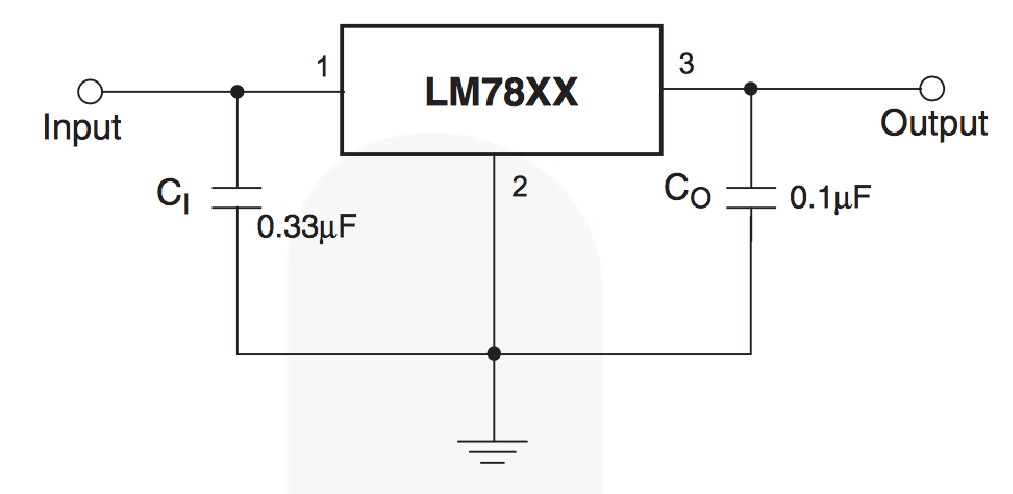
\includegraphics[width=\textwidth]{filer/design/Billeder/LM7805_DATASHEET}}
\caption{Forbindelse af LM7805 - Side 18/24 LM7805.pdf}
\label{lab:LM7805}
\raggedright
\end{figure}

Spændingsregulatoren LM7805 er opbygget i Multisim se figur \ref{lab:LM7805_SIMULERING}, sammen med 12V dc forsyningen. Kredløbet er simuleret og dette viser at outputtet er de ønskede 5 V.

\begin{figure}[H] \centering
{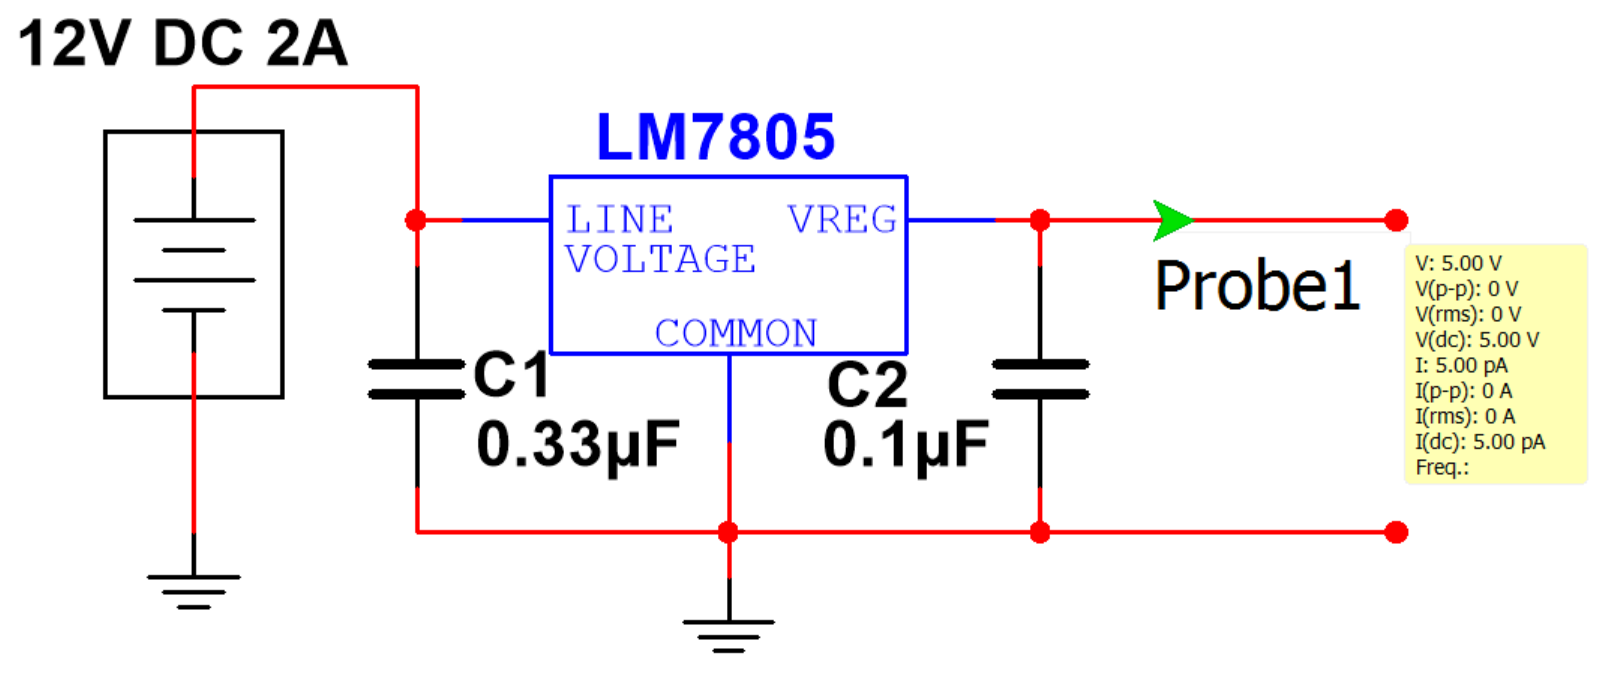
\includegraphics[width=\textwidth]{filer/design/Billeder/LM7805_SIMULATION}}
\caption{LM7805 Simulering}
\label{lab:LM7805_SIMULERING}
\raggedright
\end{figure}


For at opnå 3,3V benyttes en justerbar spændingsregulator LM317. Denne regulator kan levere 1,2V-33V 3A. Det er fugt- og temperatursensoren der skal forsynes med 3,3 V / 180 uA, det er LM317'erns opgave. 

LM317 er slået op på iPad appen "Electronic Toolbox", vha. denne gives hvordan opsætningen af denne skal være for at opnå 3,3V 
 
\begin{figure}[H] \centering
{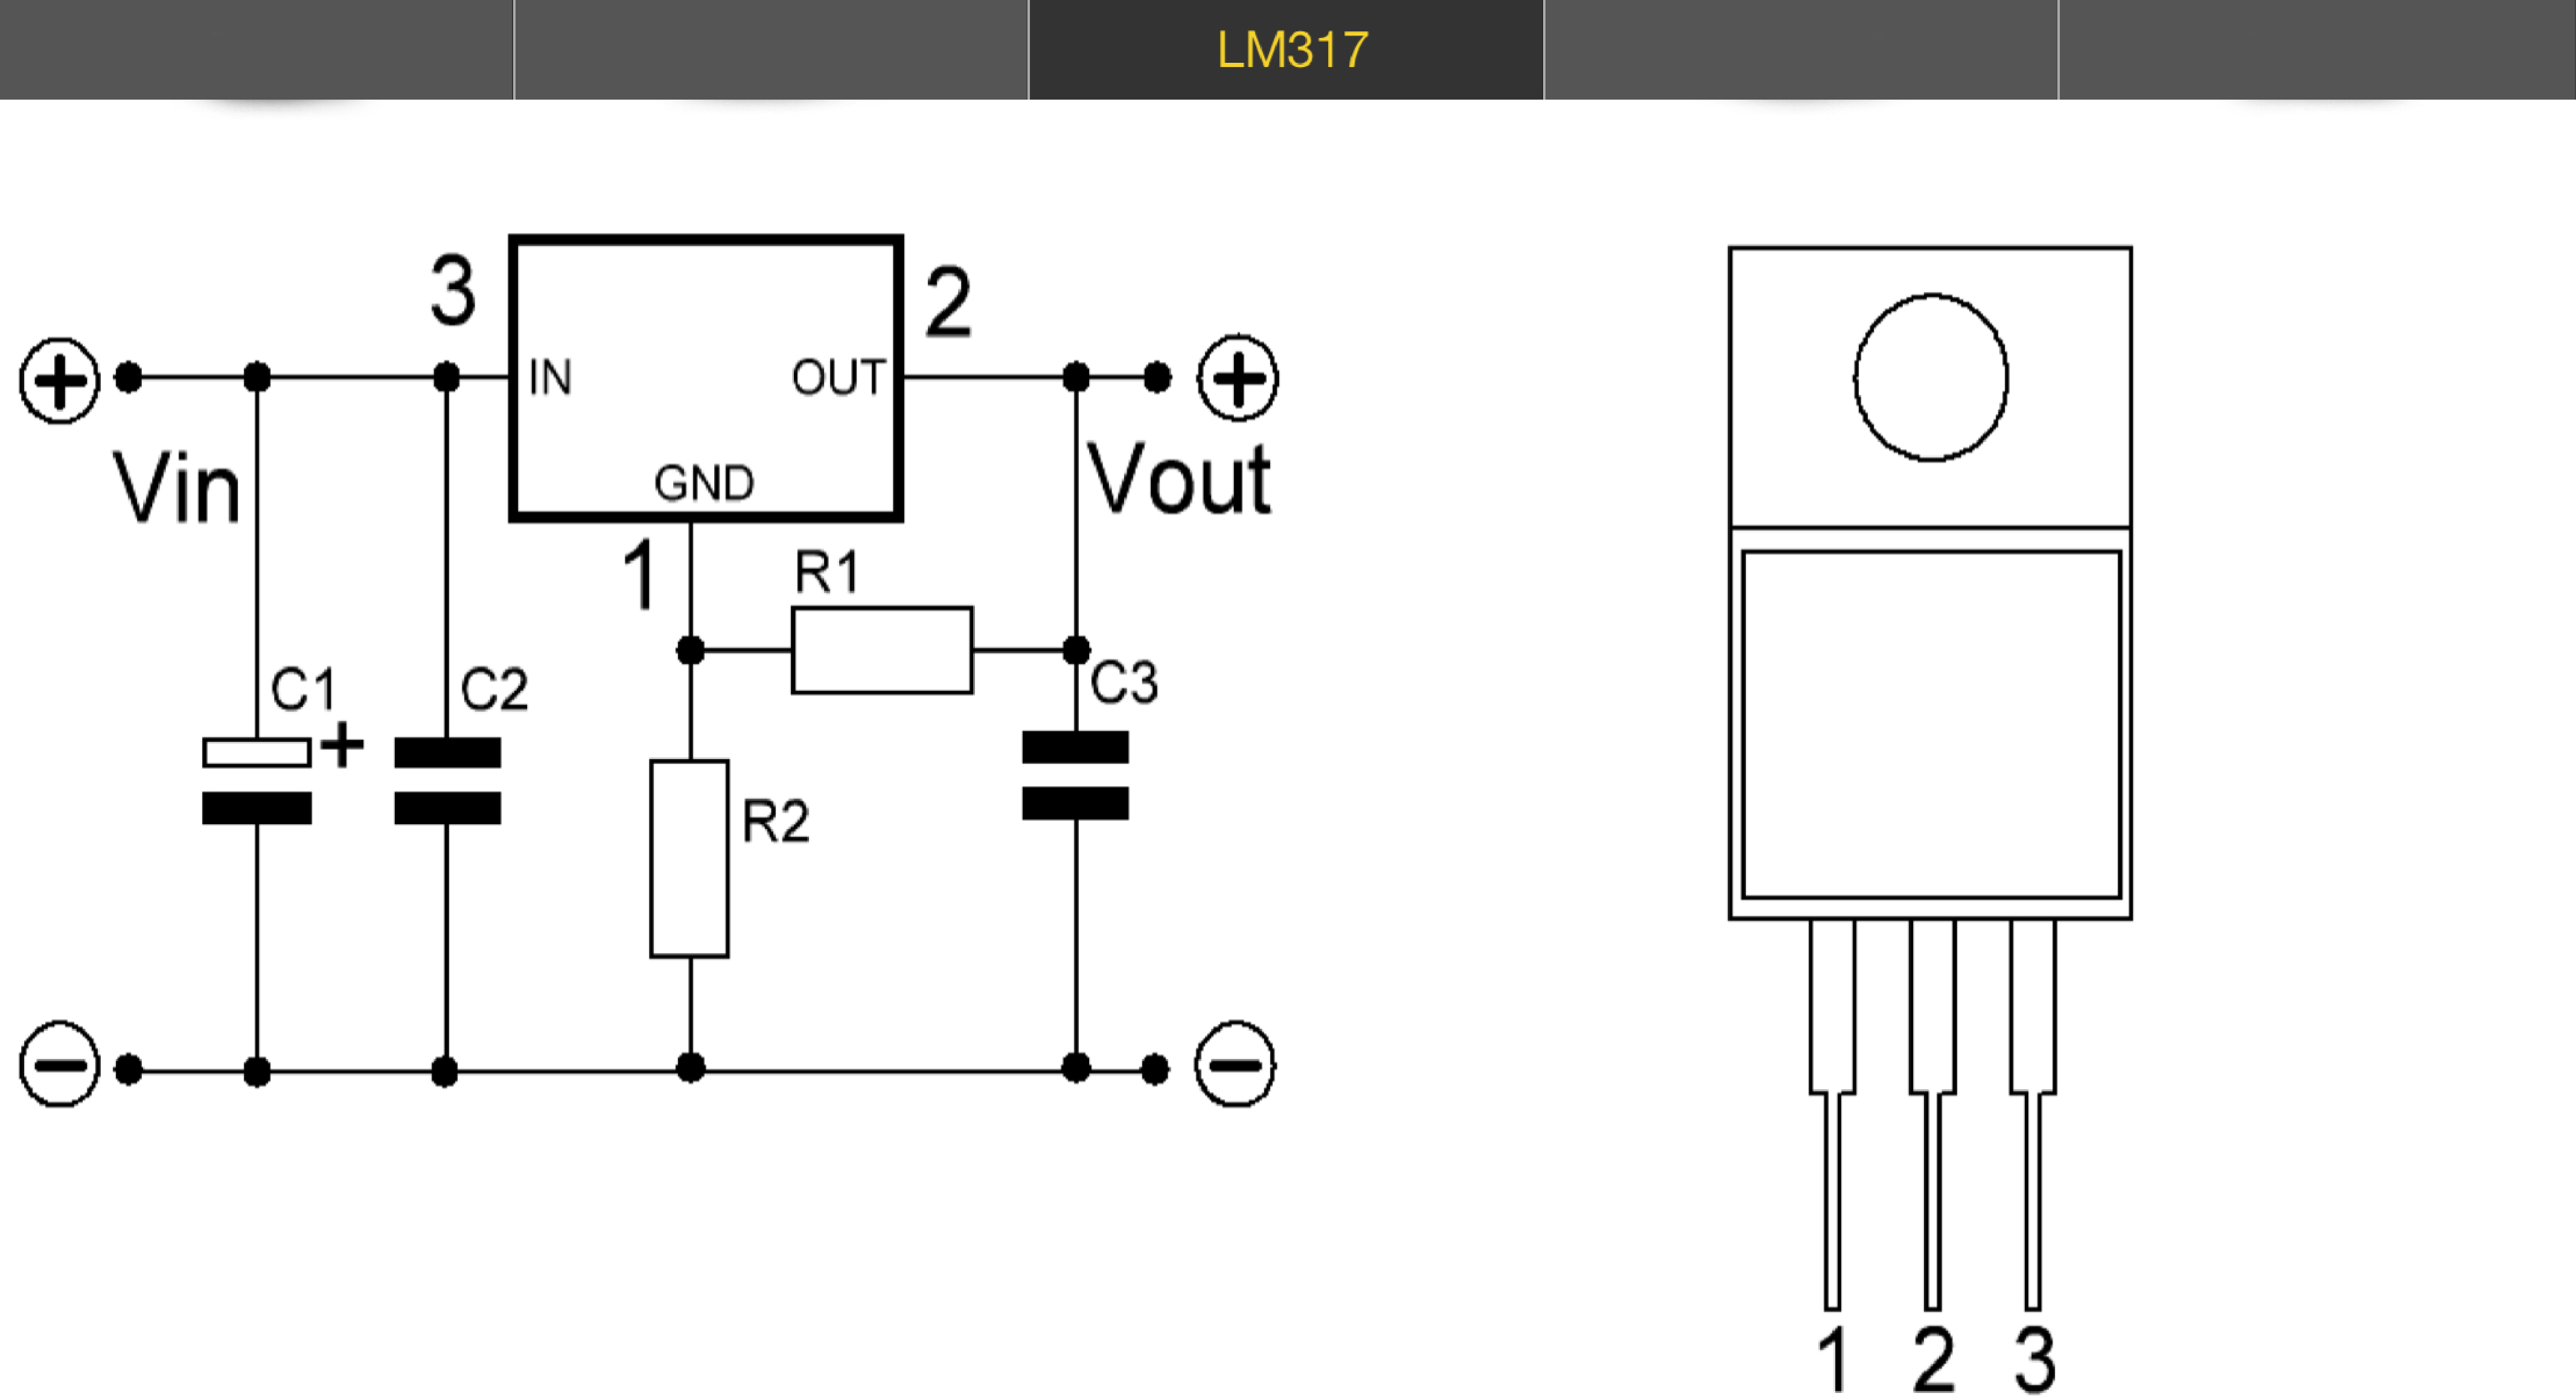
\includegraphics[width=\textwidth]{filer/design/Billeder/LM317}}
\caption{Kredsløb for LM137}
\label{lab:LM317}
\raggedright
\end{figure}

Figur \ref{lab:LM317_calc} viser hvorledes appen beregner en værdi for modstanden R2, når Vout er sat til 3,3V og modstanden R1 anbefales til 240 ohm. I følge appens beregning skal R2 være 393,6 ohm.

\begin{figure}[H] \centering
{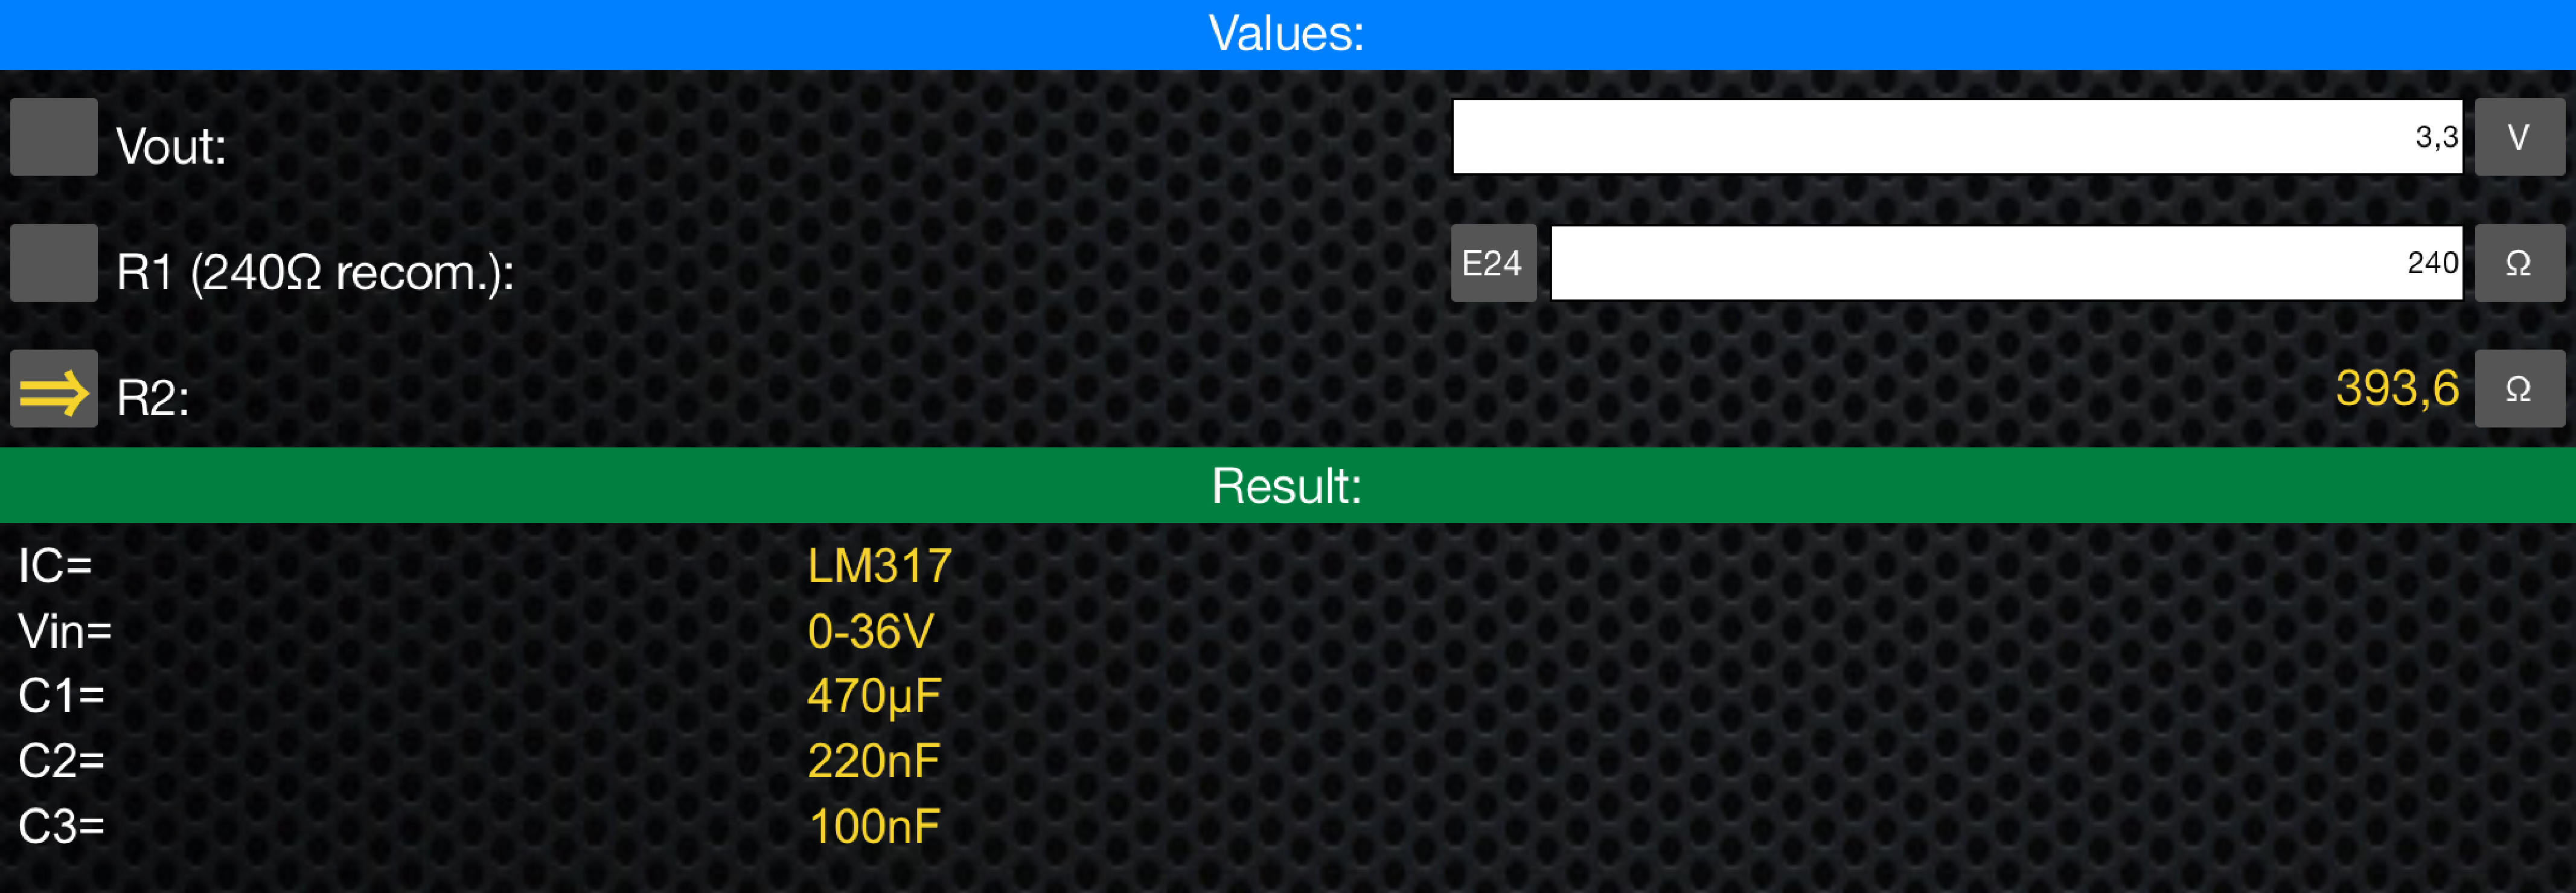
\includegraphics[width=\textwidth]{filer/design/Billeder/LM317_calc}}
\caption{Kredsløb for LM137}
\label{lab:LM317_calc}
\raggedright
\end{figure}

Det er muligt at beregne udgangsspændingen ud fra følgende formel \ref{eq:LM314_1} som er oplyst i databladet for LM317 og i Analogteknik\footnote{Analogteknik, s 259, afsnit 6.8 Serieregulator}. Strømmen $I_Q$ er strømmen der løber fra ben 1, den er mindre end 100 uA og typisk på 50 uA, de 1,25 V er spændingen imellem udgangen og referencen. Det giver følgende resultat i formlen \ref{eq:LM314_2}. 

\begin{equation} 
V_{out} = 1,25 V*(1+\frac{R2}{R1})+I_Q*R2
\label{eq:LM314_1}
\end{equation}
\begin{equation} 
V_{out} = 1,25 V*(1+\frac{390\Omega}{240\Omega})+50uA*390\Omega = 3,3 V
\label{eq:LM314_2}
\end{equation}


I formel \ref{eq:effekt_4} er der fortaget en effektberegning på LM317. Den bliver belastet med FT-sensoren som har et strømforbrug på 180 uA, plus $I_X$ som er strømmen der løber ned i modstandene. Den er fundet ved at finde strømmen der løber i R1 vha. ohms lov og ligge den sammen med strømmen fra ben 1 se \ref{eq:effekt_5}. Effektudregningen viser at det ikke er nødvendigt med køling, men der er dog  fortaget køling med køleplader alligevel. Det skyldes at det er altid en god ide at køle på et komponent hvis der er mulighed for det, det sikre bl.a længere levetid og berøringssikkerhed.

\begin{equation} 
I_X = \frac{1,25V}{250\Omega}+50uA = 5,2 mA  
\label{eq:effekt_5}
\end{equation} 
\begin{equation} 
P = (V_{DC}-V_{out})*(I_{FT-sensor}+I_X) 
\label{eq:effekt_3}
\end{equation}
\begin{equation} 
P = (12V - 3,3V)*(180 uA +5,2 mA)= 0,05 W 
\label{eq:effekt_4}
\end{equation}


Figur \ref{lab:LM317_SIMULERING} viser simuleringen af LM317 spændingsregulatoren. Outputtet er 3,3V som forventet. Der simuleres med en modstand R2 på 390 ohm og ikke 393,6 ohm.

\begin{figure}[H] \centering
{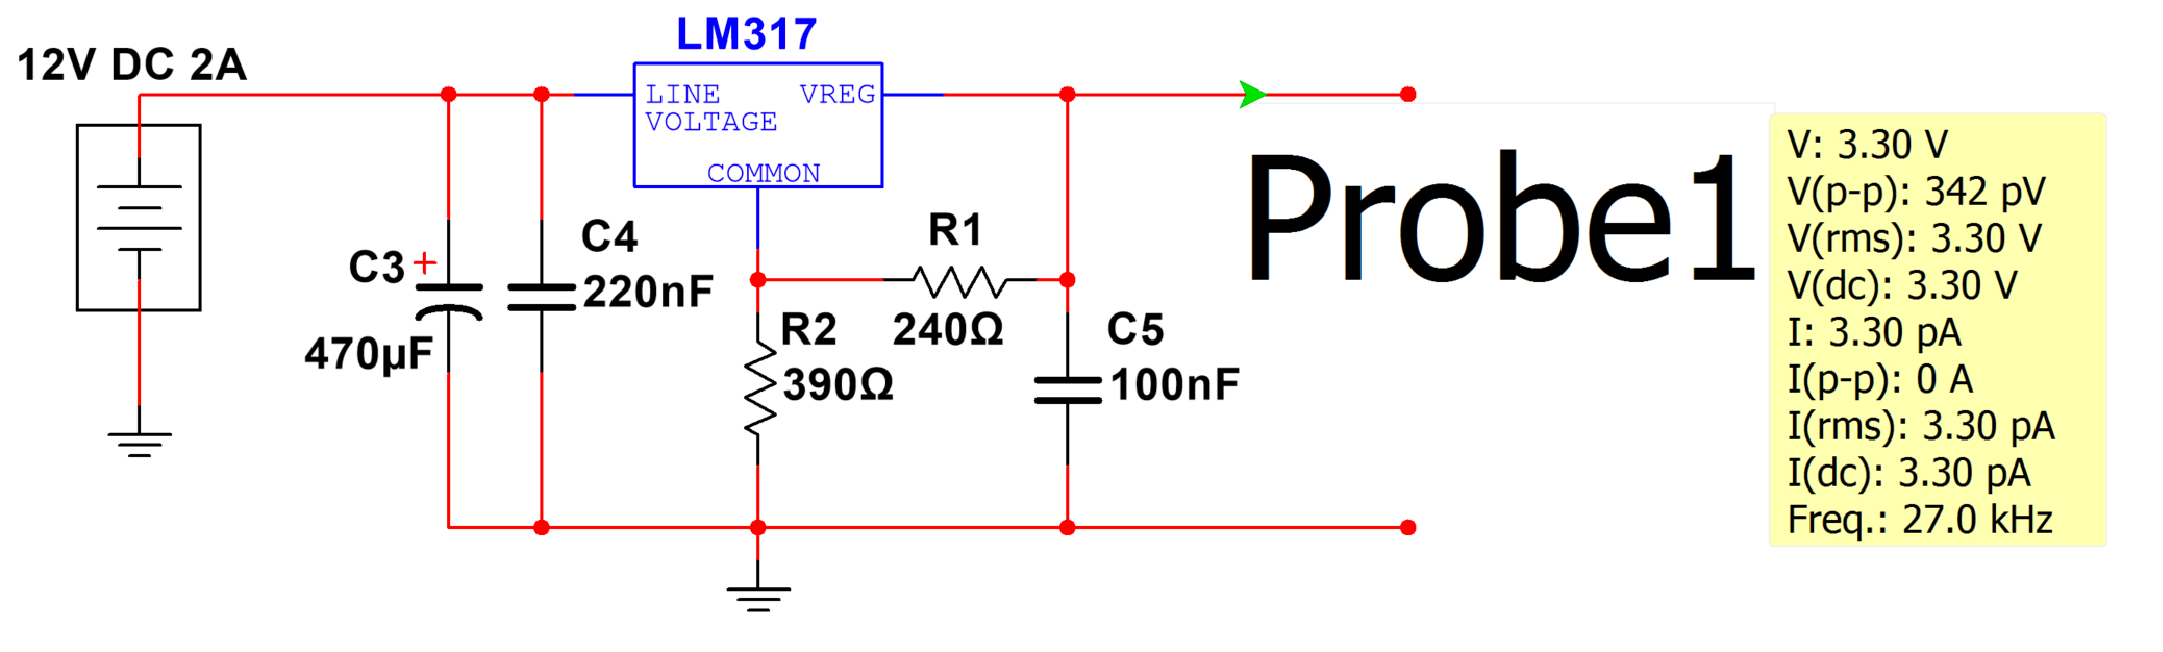
\includegraphics[width=\textwidth]{filer/design/Billeder/LM317_SIMULATION}}
\caption{Simulering i Multisim ud fra Electronic Toolbox appens værdier}
\label{lab:LM317_SIMULERING}
\raggedright
\end{figure}


\subsection{Tilslutningsprint}

Tilslutningsprintet, se figur \ref{lab:PSU_connections}, sørger for at sammenkoble Enheden med de ønskede sensorer, samt at forsyne Enhed og sensorer med ønsket forsyning.

\begin{figure}[H] \centering
{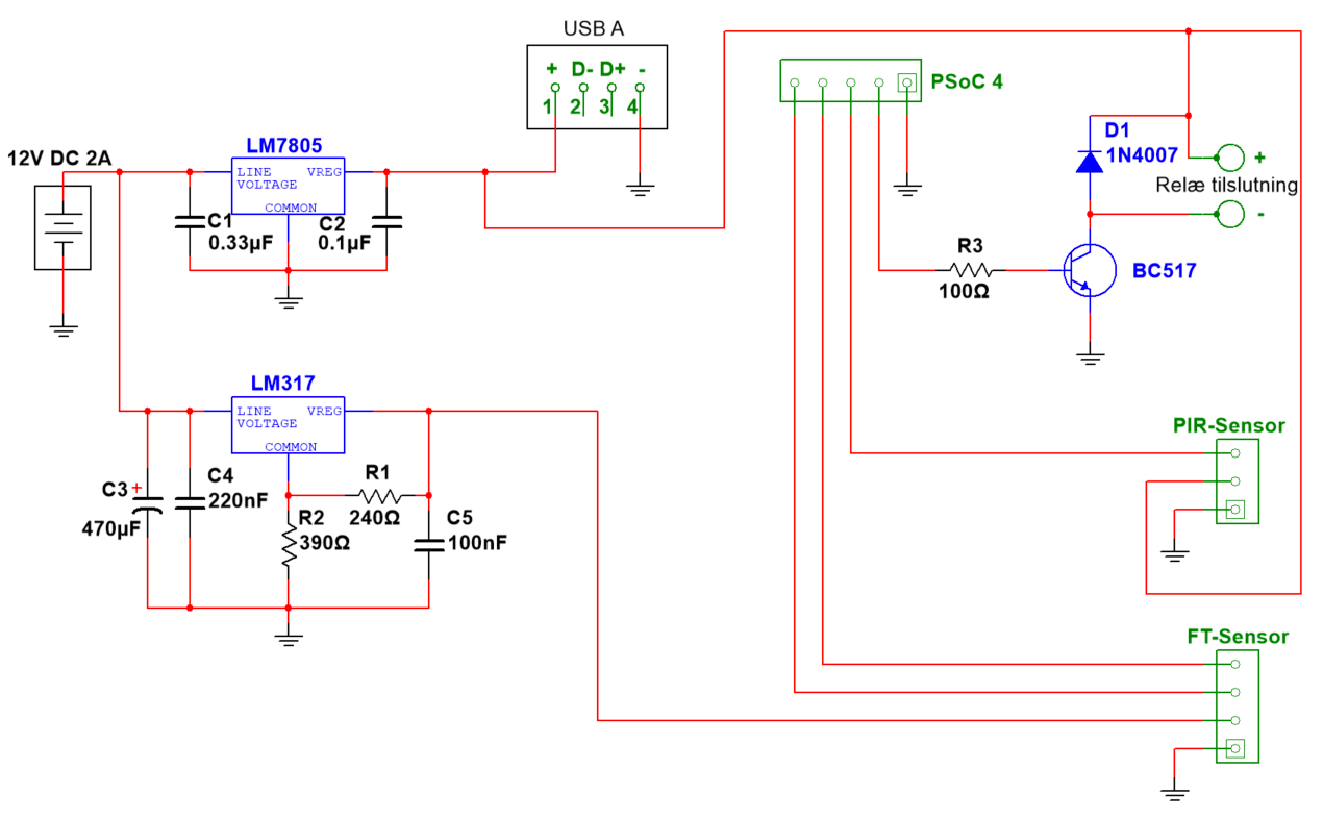
\includegraphics[width=\textwidth]{filer/design/Billeder/tilslutningsprint}}
\caption{Kredsløb over samlet spændingsforsyning (3,3V og 5V) og tilslutninger til PSoC4}
\label{lab:PSU_connections}
\raggedright
\end{figure}

